This calculator is capable of assessing the damage distribution due to a single scenario earthquake, for a collection of assets. Similarly to the previous calculator, in order to perform the necessary risk calculations one or a set of ground motion fields are required, which can be derived using the oq-hazardlib, or introduced in the OpenQuake-engine using the appropriate NRML schema.
In this calculator, a fragility model is combined with the distribution of ground motion at the location of each asset, to estimate the number or area of buildings in each damage state. The damage distribution can be extracted per asset, per building typology (taxonomy) or considering all of the assets simultaneously (total damage distribution). In addition, this calculator also provides collapse maps, which contain the spatial distribution of the number or area of collapsed buildings throughout the region of interest. The input/output structure for this calculator is presented in Figure~\ref{fig:ScnDamage}.

\begin{figure}[ht]
\centering
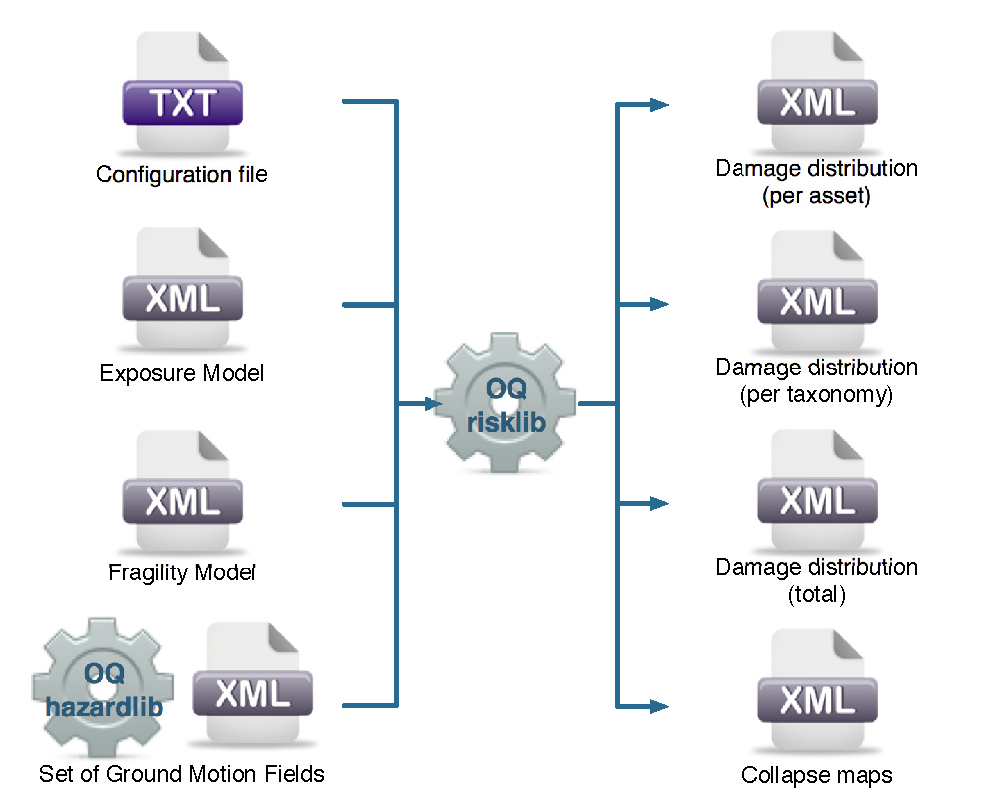
\includegraphics[width=9cm,height=7cm]{figures/risk/ScenarioDamage.pdf}
\caption{Scenario Damage Calculator input/output structure.}
\label{fig:ScnDamage}
\end{figure}